% !TeX spellcheck = en_US
\documentclass[12pt]{article}
\usepackage[T1]{fontenc}
\usepackage[utf8]{inputenc}
\usepackage{amsmath,amsthm,amsfonts,amssymb,amscd}
\usepackage[lining,semibold,scaled=1.05]{ebgaramond}     
%\usepackage[cmintegrals,cmbraces]{newtxmath}
% Use FUCKING GARAMOND
\usepackage{hyperref}
\hypersetup{
	colorlinks,
	linkcolor={red!50!black},
	citecolor={blue!50!black},
	urlcolor={blue!80!black}
}
\urlstyle{same}
\usepackage[ebgaramond]{newtxmath}
\usepackage{xparse}
\usepackage{minted}
\usepackage{graphicx}                    
% Publication quality tables          
% Driver-independent color extensions
\usepackage[margin=1in]{geometry}           
% Customize document dimensions        
% all 4 margins to be either 1 inch or 1.5 cm
\usepackage{mathtools}           

% Creating circuits        
% Print exactly what you type in
\usepackage[us]{datetime} 
% Various time format
\usepackage{blindtext}
\usepackage{bbding}
\usepackage[scr=euler,cal=dutchcal,frak=euler,bb=dsfontserif,bbsymbols]{mathalfa}
\usepackage{bbm}
\usepackage{bm}
\usepackage{multirow}
\usepackage{multicol}
\usepackage[x11names,table]{xcolor}
\usepackage[shortlabels]{enumitem}   
\usepackage{standalone}
\usepackage{microtype}
\usepackage{censor}
\usepackage[backend=biber,style=alphabetic]{biblatex}
\usepackage{courier}
\usepackage{movement-arrows}
\usepackage{algorithm}
\usepackage{algpseudocode}
\usepackage[makeroom]{cancel}
\usepackage{tcolorbox}
\tcbuselibrary{skins,raster,theorems,listings,minted}
\usepackage{mathtools}
\usepackage{soul}
\usepackage{multicol}
\usepackage{caption}
\usepackage{wrapfig}
\usepackage{authblk}
\usepackage{float}
\usepackage{fontawesome5}
\usepackage{tikz}
\usetikzlibrary{positioning}
\usetikzlibrary{shapes.geometric,arrows,patterns,arrows.meta, bending,calc,matrix, shadings,intersections,shadows,decorations,fit,backgrounds,circuits.ee.IEC,shapes.callouts}
\newcounter{dummy}



\definecolor{dkgreen}{rgb}{0,0.6,0}
\definecolor{dred}{rgb}{0.545,0,0}
\definecolor{dblue}{rgb}{0,0,0.545}
\definecolor{lgrey}{rgb}{0.9,0.9,0.9}
\definecolor{gray}{rgb}{0.4,0.4,0.4}
\definecolor{darkblue}{rgb}{0.0,0.0,0.6}
\DeclareMathOperator*{\argmax}{arg\,max}
\DeclareMathOperator*{\argmin}{arg\,min}


\renewcommand{\labelitemi}{$\textcolor{SteelBlue4}{\bullet}$}
\renewcommand{\labelitemii}{$\textcolor{blue}{\cdot}$}
\renewcommand{\labelitemiii}{$\textcolor{SkyBlue4}{\diamond}$}
\renewcommand{\labelitemiv}{$\textcolor{SkyBlue4}{\ast}$}

\newcommand{\enf}[1]{\textcolor{DodgerBlue3}{\textbf{#1}}} %enf sta per enfasi
\let\emph\enf
\newcommand{\sott}[1]{\setulcolor{SkyBlue3}\ul{#1}}
\let\underline\sott

\newcommand{\prob}{\mathbb{P}}
\newcommand\independent{\protect\mathpalette{\protect\independenT}{\perp}}
\newcommand{\ev}{\mathbb{E}}
\def\independenT#1#2{\mathrel{\rlap{$#1#2$}\mkern2mu{#1#2}}}
\newcommand{\Z}{\mathbb{Z}}
\newcommand{\R}{\mathbb{R}}
\newcommand{\N}{\mathbb{N}}
\newcommand{\T}{\mathbb{T}}
\newcommand{\Tbar}{\overline{\T}}
\newcommand{\A}{\mathscr{A}}
\newcommand{\Nstar}{\N^{*}}
\newcommand{\Rext}{\overline{\R}}
\newcommand{\io}{\text{ i.o.}}
\newcommand{\normale}{\mathcal{N}}
\newcommand{\equalexpl}[1]{%
	\underset{\substack{\uparrow\\\mathrlap{\text{\vspace{-3cm}\hspace{-1em}#1}}}}{=}}
\newcommand{\dif}{\mathop{}\!\mathrm{d}}
\newcommand{\convas}{\xrightarrow[]{\text{a.s.}}}
\newcommand{\convpr}{\xrightarrow[]{\pr}}
\newcommand{\convd}{\xrightarrow[]{\text{d}}}
\newcommand{\convlp}{\xrightarrow[]{\lp}}
\newcommand{\lone}{L^{1}}
\newcommand{\convw}{\xrightarrow[]{\mathrm{weak}}}
\newcommand{\as}{\text{ a.s.}}
\newcommand{\asstnr}{\sim N(0,1)}
%\def\checkmark{\tikz\fill[scale=0.4](0,.35) -- (.25,0) -- (1,.7) -- (.25,.15) -- cycle;} 
\newcommand{\dx}{\dif x}
\newcommand{\dy}{\dif y}
\newcommand{\dt}{\dif t}
\newcommand{\du}{\dif u}
\newcommand{\ds}{\dif s}
\newcommand{\dw}{\dif\omega}
\newcommand{\dz}{\dif z}
\newcommand{\dmu}{\dif\mu}
\newcommand{\dpr}{\dif\pr}
\newcommand{\E}{\mathscr{E}}
\newcommand{\B}{\mathscr{B}}
\newcommand{\F}{\mathscr{F}}
\newcommand{\G}{\mathscr{G}}
\newcommand{\HS}{\mathscr{H}}
\newcommand{\Zn}{\mathscr{Z}}
\newcommand{\D}{\mathscr{D}}
\newcommand{\xbar}{\overline{X}}
\newcommand{\rbar}{\overline{\R}}
\newcommand{\ybar}{\overline{Y}}
\newcommand{\xxbar}{\overline{\xbar}}
\newcommand{\xtilde}{\widetilde{X}}
\newcommand{\ifonly}{\underline{if and only if}}
\newcommand{\ang}[1]{\langle#1\rangle}

\newcommand{\ubracketthin}[1]{\underbracket[0.3pt]{#1}}

\newcommand*\circled[1]{\tikz[baseline=(char.base)]{
		\node[shape=circle,draw,
		shading=ball, ball color=SkyBlue1!70,
		,inner sep=1.5pt] (char) {\scriptsize\bfseries #1};}}
\newcommand{\circnum}{\protect\circled{\arabic*}}
\newcommand{\circlet}{\protect\circled{\alph*}}	
\newcommand{\bbg}[1]{%
	\ooalign{$#1$\cr\raisebox{-.2pt}{$#1$}\cr\raisebox{.2pt}{$#1$}\cr\textcolor{white}{$\mkern0.2mu#1$}}%
}
\newcommand{\leb}{\bbg{\lambda}}

%i comandi di MERDA di stefano
\newcommand{\ra}{\rightarrow}
\newcommand{\iy}{\infty}
\newcommand{\mE}{\mathbb{E}}
\newcommand{\mP}{\mathbb{P}}
\newcommand{\mB}{\mathcal{B}(\mathbb{R})}
\newcommand{\mL}{\mathbb{L}}
\newcommand{\ninfty}{n\to$\infty$}
\newcommand{\tinfty}{t\to$\infty$}
\newcommand{\xinfty}{x\to$\infty$}
\newcommand{\yinfty}{y\to$\infty$}
\newcommand{\mLL}{\mathbb{L}^2(0,T)}
\newcommand{\mR}{\mathbb{R}}
\newcommand{\mC}{\mathcal{C}}
\newcommand{\mRd}{\mathbb{R}^d}
\newcommand{\mN}{\mathbb{N}}
%\newcommand{\m1}{\mathbf{1}}
\newcommand{\mF}{\mathcal{F}}
\newcommand{\mM}{\mathcal{M}}
\newcommand{\mW}{\mathcal{W}}
\newcommand{\mV}{\mathcal{V}}
\newcommand{\mA}{\mathcal{A}}
\newcommand{\mez}{\frac{1}{2}}
\newcommand{\intT}{\int_{0}^{T}}
\newcommand{\nN}{n \in \mathbb{N}}
\newcommand{\mmN}{\mathcal{N}}
\newcommand{\BM}{(B_t)_{t\geq 0}}
\newcommand{\PX}{(X_t)_{t\geq 0}}
\newcommand{\var}{\mathbb{V}\!\mathrm{ar}\,}
\newcommand{\cov}{\mathbb{C}\mathrm{ov}\,}
\newcommand{\lp}{L^{p}}
\newcommand{\BMF}{\left((B_t)_{t\geq 0},\mathcal{F}_t \right)}
\newcommand{\mFt}{\mathcal{F}_t}
\newcommand{\every}{\forall\,}
\newcommand{\dyadic}{\mathcal{d}}
\newcommand{\norm}[1]{\left|\negthinspace\left|#1\right|\negthinspace\right|}
\newcommand{\pr}{\mathbb{P}}
\newcommand{\indi}{\mathbb{1}}
\newcommand{\trns}[1]{{#1}^{\scriptscriptstyle\mathsf{T}}}
\newcommand{\iid}{\stackrel{\mathrm{iid}}{\sim}}
\newcommand{\unmezz}{\frac{1}{2}}
\newcommand{\sa}{$\sigma$-algebra}	\newcommand{\rv}{random variable}
\newcommand{\prefacename}{Preface}
\newcommand{\cinlar}{Çinlar }
\newenvironment{preface}{
	\vspace*{\stretch{2}}
	{\noindent \bfseries \huge\color{SkyBlue4} \prefacename}
	\begin{center}
		% \phantomsection \addcontentsline{toc}{chapter}{\prefacename} % enable this if you want to put the preface in the table of contents
		\thispagestyle{plain}
	\end{center}%
}
{\vspace*{\stretch{5}}}


\newenvironment{closethedeal}{
	\vspace*{\stretch{2}}
	{\noindent \bfseries \huge\color{SkyBlue4} That's all, folks}
	\begin{center}
		% \phantomsection \addcontentsline{toc}{chapter}{\prefacename} % enable this if you want to put the preface in the table of contents
		\thispagestyle{plain}
	\end{center}%
}
{\vspace*{\stretch{5}}}
\pgfkeys{%
	/calloutquote/.cd,
	width/.code                   =  {\def\calloutquotewidth{#1}},
	position/.code                =  {\def\calloutquotepos{#1}}, 
	author/.code                  =  {\def\calloutquoteauthor{#1}},
	/calloutquote/.unknown/.code   =  {\let\searchname=\pgfkeyscurrentname
		\pgfkeysalso{\searchname/.try=#1,                                
			/tikz/\searchname/.retry=#1},\pgfkeysalso{\searchname/.try=#1,
			/pgf/\searchname/.retry=#1}}
}  


\newcommand\calloutquote[2][]{%
	\pgfkeys{/calloutquote/.cd,
		width               = 5cm,
		position            = {(0,-1)},
		author              = {}}
	\pgfqkeys{/calloutquote}{#1}                   
	\node [rectangle callout,draw,callout relative pointer={\calloutquotepos},text width=\calloutquotewidth,/calloutquote/.cd,
	#1] (tmpcall) at (0,0) {#2};
	\node at (tmpcall.pointer){\calloutquoteauthor};    
}  		


\newcommand\lemmethink[2][]{%
	\pgfkeys{/calloutquote/.cd,
		width               = 5cm,
		position            = {(0,-1)},
		author              = {}}
	\pgfqkeys{/calloutquote}{#1}                   
	\node [cloud callout,draw,callout relative pointer={\calloutquotepos},text width=\calloutquotewidth,/calloutquote/.cd,
	#1] (tmpcall) at (0,0) {#2};
	\node at (tmpcall.pointer){\calloutquoteauthor};    
}  											


\renewcommand\leq\leqslant
\renewcommand\geq\geqslant		
\setlength\parindent{0pt}

%%%%%%%%%%%%%%%%%%%%%%%%%%%%%%%%%%%%%%%%%%%%%%%%%%%%%%%%%%%%%%
%%%%%%%%%%%%%%%%%%%%%%%%%%%%%%%%%%%%%%%%%%%%%%%%%%%%%%%%%%%%%%
\usemintedstyle{monokai}
\definecolor{codeBg}{HTML}{282822}
\newenvironment{py}
{\VerbatimEnvironment
	\begin{minted}[
		bgcolor=codeBg,
		breaklines,
		fontsize=\footnotesize
		]
		{python}}
	{\end{minted}}

	%\newmintinline[bluecode]{c++}{\color{codeblue}}
	
\newcommand{\pyinl}[1]{\mintinline[bgcolor=black!40]{python}{#1}}
%%%%%%%%%%%%%%%%%%%%%%%%%%%%%%%%%%%%%%%%%%%%%%%%%%%%%%%%%%%%%%

%%%%%%%%%%%%%%%%%%%%%%%%%%%%%%%%%%%%%%%%%%%%%%%%%%%%%%%%%%%%%%%
\definecolor{UM_Brown}{HTML}{3D190D}
\definecolor{UM_DarkBlue}{HTML}{2264B0}
\definecolor{UM_LightBlue}{HTML}{1CA9E1}
\definecolor{UM_Orange}{HTML}{fEB415}
\addbibresource{biblio.bib}




\tikzstyle{startstop} = [rectangle, rounded corners, minimum width=3cm, minimum height=1cm,text centered, draw=black, fill=red!30]
\tikzstyle{io} = [trapezium, trapezium left angle=70, trapezium right angle=110, minimum width=3cm, minimum height=1cm, text centered, draw=black, fill=blue!30]
\tikzstyle{process} = [rectangle, minimum width=3cm, minimum height=1cm, text centered, draw=black, fill=orange!30]
\tikzstyle{decision} = [diamond, minimum width=3cm, minimum height=1cm, text centered, draw=black, fill=green!30]
\tikzstyle{arrow} = [thick,->,>=stealth]

\begin{document}
	\textcolor{UM_Brown}{
		\begin{center}
			\textbf{\Large Simulations}\\
			\vspace{5pt}
			Homework 7 \\
			\vspace{5pt}
			\textbf{M.S. in Stochastics and Data Science}\\
			\vspace{20pt}
			\textit{Andrea Crusi, Lorenzo Sala} \\
			\vspace{5pt}
			\today
		\end{center}
		\vspace{10pt}
		\hrule
	}
	
	
	
	
	%%%%%%%%%%%%%%% NEW SECTION %%%%%%%%%%%%%%% 
	\section{Exercise 1}
	\subsection{Overview}
	We start this discussion by taking a look at the main characteristics of the network of queues in question.\\
	In this system we have $N=10$ machines departing from the ``delay station'' $Z$ with a certain rate (which is modeled by a random variable $Z$); from here they reach a short repair station where they undergo a short reparation whose duration is another random variable $X$; finally, with a probability $\beta=0.2$ they reach a long repair station where the duration of the repair is yet another random variable $Y$. The machines that do not go the the long repair station or that have finished the long repair go back to the source.
	In this case the distribution of all the three stations is \emph{negative exponential distributions}:
	\begin{equation*}
		F_X(x)=\pr(X\leq x)=1-e^{-\frac{1}{\eta} x}\qquad f_X(x)=\frac{\dif F_X}{\dx}=\lambda e^{-\frac{1}{\eta} x}.
	\end{equation*}
	In this formulation the parameter is given directly as the expected value $\ev[X]=\eta$ of the distribution. We have our three expected values, reflecting the average time of each of these three events:
	\begin{enumerate}[\circnum]
		\item time between breakages of a machine: $\eta_{\mathsf{arrival}}=3000\text{ mins}$;
		\item service time of the short repair station: $\eta_{\mathsf{short}}=40\text{ mins}$;
		\item service time of the long repair station: $\eta_{\mathsf{long}}=960\text{ mins}$.
	\end{enumerate}
	This characteristic brings us to the particular case of the tandem server with ``M/M/2'' service and arrival times seen during lectures. 
In this scenario, due to the memoryless property of the negative exponential distribution for all time variables (e.g., failure times, short and long repair times), defining regeneration points is straightforward. For example, a regeneration point can be set as the time when a machine enters the long repair station and the system resets to its initial conditions. This choice is based on the following schema:
		
		\begin{table}[H]
			\centering
			\renewcommand{\arraystretch}{1.5}
			\begin{tabular}{|m{4cm}|m{4cm}|m{4cm}|}
				\hline
				\multicolumn{1}{|c|}{\textbf{Service time distribution of the first queue}} &
				\multicolumn{2}{c|}{\textbf{Service time distribution of the second queue}} \\ 
				\cline{2-3}
				& \textbf{GENERIC} & \textbf{MARKOV (Neg-Exp)} \\ 
				\hline
				\textbf{GENERIC} & Any departure that leaves behind exactly $N - 1$ customers from one of the two servers of the network & Any departure from the first server \\ 
				\hline
				\textbf{MARKOV (Neg-Exp)} & Any departure from the second server & Any departure in the system \\ 
				\hline
			\end{tabular}
			\caption{Service time distribution schema for the first and second queue.}
			\label{table1}
		\end{table}
	in which we can easily notice we are in the bottom-right case, in which the service times of both the queue are negative-exponential.\\
	Technically every departure could be a regeneration point but since our analysis focuses on the average waiting time of the long repair station we chose as regeneration points all the departures from the long station. 
	This choice will also simplify our calculations: the value $\nu_{j}$, that counts the number of the occurrences of the event of interest in the current regeneration cycle, will always be 1. \\
	For the distribution of the routings we assume a uniform distribution (so that 20\% of the departures from the short station will become an arrival to the long station).
	\subsection{The simulation}
	For the implementation of this simulation we chose the classic event list approach: the bulk of the simulator is an ever-growing list of events sorted by the timestamp of their occurrence. Each of these events is ``processed'' one by one, typically by adding another related event to the list and computing the necessary measurements. \\
	To implement the regeneration method, we will keep track of the measurements of interest for each cycle $j$ (like the total waiting time at a certain station $A_{j}$ and the count $\nu_{j}$ of events happened during that cycle) and once we meet a regeneration point we accumulate those measures in global cumulative variables before resetting them and starting over.
	\begin{figure}[h]
		\centering
			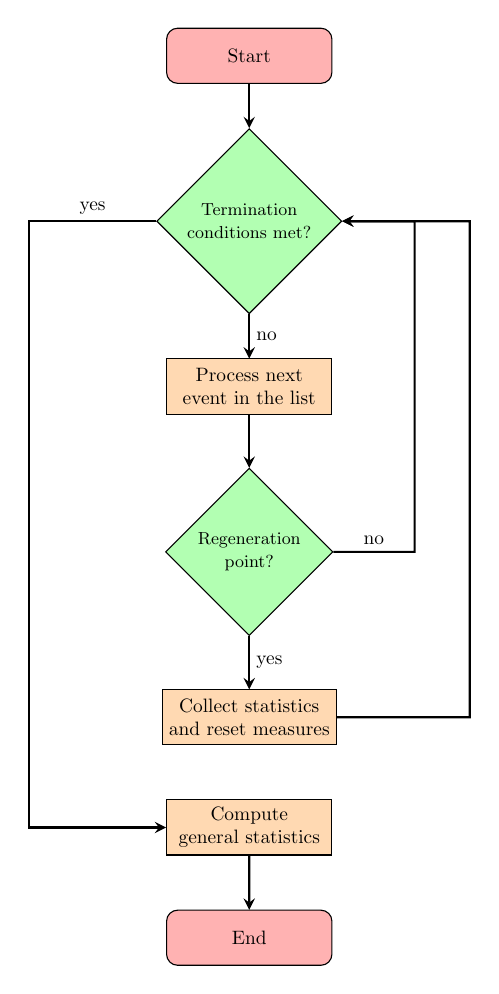
\begin{tikzpicture}[scale=0.7, every node/.style={scale=0.7},node distance=2cm]
			\node (start) [startstop] {Start};
			\node (conditions) [decision, align=center, below of=start,yshift=-1cm] {\small Termination \\ \small conditions met?};
			\node (mainloop) [process,below of=conditions,yshift=-1cm,align=center] {Process next \\ event in the list};
			\node (regen) [decision, align=center, below of=mainloop,yshift=-1cm] {\small Regeneration\\ \small point?};
			\node (collect) [process, below of=regen, yshift=-1cm,align=center]{Collect statistics \\ and reset measures};
			\node (terminate) [process, below of=collect,align=center]{Compute\\ general statistics};
			\node (end) [startstop,below of=terminate] {End};
			\draw [arrow] (start)--(conditions);
			\draw [arrow] (conditions)--node[anchor=south]{yes}+(-4,0)|- (terminate);
			\draw [arrow] (conditions)--node[anchor=west]{no}(mainloop);
			\draw[arrow] (mainloop)--(regen);
			\draw[arrow] (regen)--node[anchor=west]{yes}(collect);
			\draw[arrow] (regen)--node[anchor=south]{no}+(3,0)|-(conditions);
			\draw[arrow](collect)--+(4,0)|-(conditions);
			\draw[arrow](terminate)--(end);
		\end{tikzpicture}
		\caption{Flowchart of the operations of our simulator.}
	\end{figure}
	First of all, we definite a structure to handle each entry of our event list:
\begin{lstlisting}
typedef struct Event {
	int machine; // this will identify what machine we are talking about.
	char type;   // 'A' for Arrival, 'S' for Departure (Short Station), 'L' for
	// Departure (Long Station)
	double timestamp; // The time the event occurs
} Event;
\end{lstlisting}
By doing this we can always keep track of the information of each event that will help us determine what will happen next. We then initialize our event list.
\begin{lstlisting}
	Event *event_list = NULL; // Pointer to the array of events
	size_t event_count = 0;   // Number of events currently in the list. This will
	// grow as we add more events.
	size_t event_capacity =
	0; // This is how much memory we have allocated for this array. When the
	// list is full we need ro realloc an expanded version of this array.
\end{lstlisting}
We are going to use a dynamic array which whose size we are going to increase whenever needed. \\
Each time we want to add an element to our event list we call this function:
\begin{lstlisting}
void add_event(Event new_event) {
	// Check if resizing is needed
	if (event_count == event_capacity) {
		size_t old_capacity = event_capacity;
		event_capacity = (event_capacity == 0) ? 10 : event_capacity * 2;
		Event *temp_list = realloc(event_list, event_capacity * sizeof(Event));
		if (!temp_list) {
			fprintf(stderr, "Memory allocation failed!\n");
			exit(EXIT_FAILURE);
		}
		event_list = temp_list;
		
		// Initialize the newly allocated memory
		for (size_t i = old_capacity; i < event_capacity; i++) {
			event_list[i].machine = 0;
			event_list[i].type = '\0';
			event_list[i].timestamp = 0.0f;
		}
	}
	
	// Add the new event to the list (temporarily at the end)
	event_count++;
	event_list[event_count - 1] = new_event;
	
	// Sort the event list (insertion sort)
	size_t i = event_count - 1;
	while (i > 0 && event_list[i - 1].timestamp > event_list[i].timestamp) {
		Event temp = event_list[i];
		event_list[i] = event_list[i - 1];
		event_list[i - 1] = temp;
		i--;
	}
}
\end{lstlisting}
Here the first chunk of the code handles the dynamic resizing of the array to take into account new events added to the event list and initializes the new placeholder events; the second half of the code inserts the event at the end of the list and then performs an insertion sort to ensure the event reaches its correct placement inside the event list. This allows us to know that after inserting an event the event list will always be correctly ordered. \par
Before going to the engine of the simulation, we define some helper functions:
\begin{lstlisting}
int RegPoint(Event current_event) {
	// Regeneration point occurs at a S or L event
	// Returns 1 (true) for regeneration point, 0 (false) otherwise
	return (current_event.type == 'L');
}
\end{lstlisting}
This is a simple function that checks whether the event that we are processing is a regeneration point. In this case it is quite an easy call, since all \verb*|'L'| (departure from long repair station) events are regeneration points.
\begin{lstlisting}
void CollectRegStatistics(double *wait_currentcycle_short_station,
double *wait_currentcycle_long_station,
double *accumulated_wait_short,
double *accumulated_wait_long, int *cycle_count) {
	*accumulated_wait_short +=
	*wait_currentcycle_short_station; // Accumulate waiting time for short
	// station
	*accumulated_wait_long +=
	*wait_currentcycle_long_station; // Accumulate waiting time for short
	// station
	(*cycle_count)++;                     // Increment the cycle count
}
\end{lstlisting}
After encountering a regeneration point, this function collects the cycle-specific measures \path{wait_currentcycle_short_station} (which is the cumulative waiting time during cycle $j$ at the short repair station) and \path{wait_currentcycle_long_station} (similarly, the waiting time at the long repair station during cycle $j$) into global accumulators for later computations. Moreover, this function is also responsible to increase the counter of how many cycle have passed.
\begin{lstlisting}
void ResetMeasures(double *wait_currentcycle_long_station,
double *wait_currentcycle_short_station) {
	*wait_currentcycle_short_station =
	0.0; // Reset the cycle-specific waiting time
	*wait_currentcycle_long_station =
	0.0; // Reset the cycle-specific waiting time
}
\end{lstlisting}
This function simply resets the cycle-specific measure we talked about before.
\begin{lstlisting}
int DecideToStop(int cycle_count, double error_percentage,int iteration_number) {
	return ((cycle_count>40 && error_percentage<0.10)||iteration_number>MAX_EVENTS);
}
\end{lstlisting}
This is another simple functions like \path{RegPoint} that checks whether the termination conditions are reached. In our case, we decided to continue the simulation until one of these two conditions is reached:
\begin{enumerate}
	\item we surpass 40 cycles (so that we find ourselves in a setting in which the T-statistic converges towards the normal distribution) \underline{\textit{and}} our error is less than 10\% of our point estimate for the mean waiting time at the long station;
	\item we surpass an arbitrary threshold \path{MAX_EVENTS} to avoid the code to execute itself ad infinitum.
\end{enumerate}
\begin{lstlisting}
double ComputeConfidenceIntervals(double mean_wait_long, double time_events_product_long, double L_event_count, double accumulated_wait_long_squared, int cycle_count) {
	double S_A=accumulated_wait_long;
	double S_nu=L_event_count;
	double S_AA=accumulated_wait_long_squared;
	double S_Anu=time_events_product_long;
	double S_nunu=L_event_count; // every cycle has nu=1 so the sum of the squared nu is just the event count
	double r_hat=S_A/S_nu;
	double delta = sqrt(cycle_count/(cycle_count-1))*(sqrt(S_AA-2*r_hat*S_Anu+pow(r_hat,2)*S_nunu)/S_nu);
	double error = 1.96*delta;
	//printf("Error=%f\n",error);
	return error;
}
\end{lstlisting}
This function computes the confidence intervals for the point estimator of the average waiting time at the long station $\hat{r}$. Remember that the confidence interval at the level $(1-\alpha)$ for $r$ can be expressed as
\begin{equation*}
	\hat{r}-t_{p-1,\alpha/2}\Delta\leq r\leq\hat{r}+t_{p-1,\alpha/2}\Delta
\end{equation*} 
where
\begin{align*}
	p&=\text{ number of regeneration cycles}\\
	\Delta&=\frac{\hat{s}_{Z}}{\overline{\nu}\sqrt{p}}.
\end{align*}
where $\hat{s^{2}_{Z}}$ is the sample standard deviation of the auxiliary variable $Z_j=A_j-r\nu_j$ (used to construct the \rv{} $\frac{\overline{Z}}{\sigma_{Z}/\sqrt{p}}\sim\mathscr{N}(0,1)$) and $\overline{\nu}$ is the average number of occurrences of the event of interest in each cycle $\frac{1}{n}\sum_{j=1}^{n}\nu_j$ (that in our case, since $\nu_j=1\;\every j$ by design, will always be equal the the number of cycles).\\
Luckily, we do not have to keep track of each single waiting time or occurrence count, since we know that we can express $\Delta$ as
\begin{equation*}
	\Delta=\sqrt{\frac{p}{p-1}}\cdot\frac{\sqrt{\hat{\mathcal{S}}_{AA}-2\hat{r}\hat{\mathcal{S}}_{A\nu}+\hat{r}^{2}\hat{\mathcal{S}}_{\nu\nu}}}{\hat{\mathcal{S}}_{\nu}}
\end{equation*}
where
\begin{align*}
	\hat{\mathcal{S}}_{AA}&=\sum_{j=1}^{p}A^{2}_{j}\\
	\hat{\mathcal{S}}_{A\nu}&=\sum_{j=1}^{p}A_j\nu_j\\
	\hat{\mathcal{S}}_{\nu\nu}&=\sum_{j=1}^{p}\nu_j^2\\
	\hat{\mathcal{S}}_{\nu}&=\sum_{j=1}^{p}\nu_j
\end{align*}
which are all quantities we can easily accumulate each time we process an event. Moreover, since by design we always go further 40 cycles, we can ditch the T-statistic and directly use the (bi-lateral) 95\% quantile from the normal standard distribution $-z_{0.05/2}=1.96$. So, in the end, we will have that
\begin{align*}
	&\pr\left(\hat{r}-1.96\cdot\sqrt{\frac{p}{p-1}}\cdot\frac{\sqrt{\hat{\mathcal{S}}_{AA}-2\hat{r}\hat{\mathcal{S}}_{A\nu}+\hat{r}^{2}\hat{\mathcal{S}}_{\nu\nu}}}{\hat{\mathcal{S}}_{\nu}}\leq r\leq\hat{r}+1.96\cdot\sqrt{\frac{p}{p-1}}\cdot\frac{\sqrt{\hat{\mathcal{S}}_{AA}-2\hat{r}\hat{\mathcal{S}}_{A\nu}+\hat{r}^{2}\hat{\mathcal{S}}_{\nu\nu}}}{\hat{\mathcal{S}}_{\nu}} \right)\\
	&\approx(1-\alpha)=0.95.
\end{align*}
We also need a way to generate our exponential random variable. Since we explicitly know the formula of the cumulative distribution function of the exponential distribution, we can use the \emph{inverse transformation method} to transform uniform random variables into exponential random variables. In this case, if $X\sim\mathsf{Exp}(\eta)$ then we can compute the inverse distribution function by solving the cumulative distribution function for $x$:
\begin{equation*}
	x=F^{-1}(u)=-\eta\ln(1-u)\qquad0<u<1.
\end{equation*}
So choosing $u\sim\mathsf{Unif}(0,1)$ and plugging it into the inverse distribution function we can obtain a \rv{} that is drawn from the exponential distribution.
\begin{lstlisting}
double exponential_random(double heta) {
	double unif = (double)rand() / RAND_MAX;
	if ((1 - unif) < 1e-20) {
		unif = 1e-20; // this will give us a limit in the case in which the argument
		// of the logarithm is too close to 0 (and thus exploding)
	}
	double exp = (-heta * logf(1 - unif));
	// double pick = 1- ((double)rand() / RAND_MAX);
	verbose ? printf("This time I extracted %f!\n", exp) : 0;
	return exp;
}
\end{lstlisting}
Here we needed to take a little safety measure since drawing uniform samples very close to 1 would sometimes cause the logarithm to explode to $\infty$. By enforcing a lower bound we may lose some accuracy in our model but at least we don't end up with infinity values.\par
Now we are ready to tackle the main engine of the simulator, which is the \path{process_event} function. We thought about this function as cursor that traverses the event list item by item and schedules one or more event according to what type of event we are processing and which machine is involved. 
\begin{figure}[h]
	\centering
	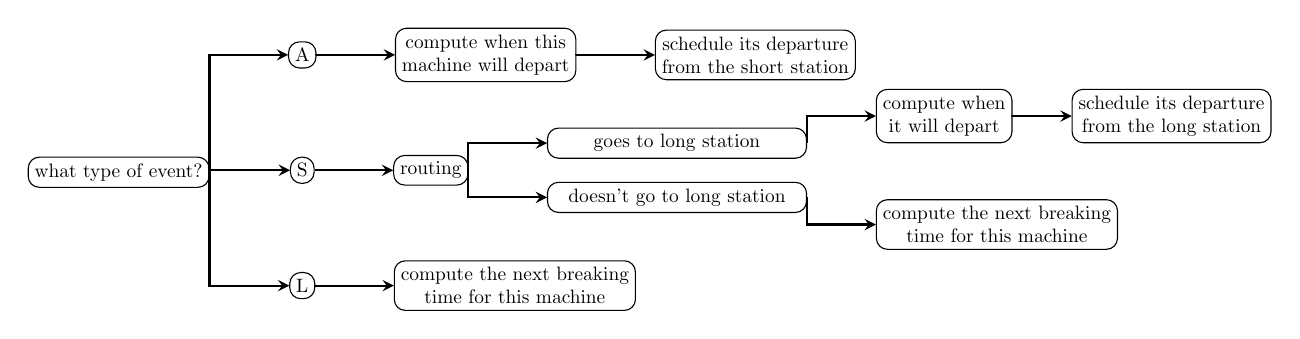
\begin{tikzpicture}[scale=0.7, every node/.style={scale=0.7}]
		\node[rectangle,rounded corners,draw](iniz){what type of event?};
		\node[rectangle,rounded corners,draw,above right=of iniz,yshift=5pt] (A) {A};
		\node[rectangle,rounded corners,draw,below=of A,yshift=-5pt] (S) {S};
		\node[rectangle,rounded corners,draw,below=of S,yshift=-5pt] (L) {L};
		\node[rectangle,draw,rounded corners,right=of A,align=center] (A1) {compute when this \\ machine will depart};
		\node [rectangle,draw,rounded corners,right=of A1,align=center] (A2) {schedule its departure\\ from the short station} ;
		\node [rectangle,draw,rounded corners,right=of S,align=center] (S1) {routing};
		\node [rectangle,draw,rounded corners,right=of S1,align=center,yshift=14pt,minimum width=4.7cm](S21){goes to long station};
		\node [rectangle,draw,rounded corners,right=of S1,align=center,minimum width=4.7cm,yshift=-14pt](S22){doesn't go to long station};
		\node [rectangle,draw,rounded corners,right=of S21,align=center,yshift=14pt,xshift=-5pt] (S31) {compute when \\ it will depart};
		\node [rectangle,draw,rounded corners,right=of S31,align=center,xshift=-10pt] (S41) {schedule its departure\\ from the long station};
		\node [rectangle,draw,rounded corners,right=of S22,align=center,yshift=-14pt,xshift=-5pt] (S32) {compute the next breaking\\ time for this machine};
		\node[rectangle,rounded corners,draw,right=of L,align=center] (L1) {compute the next breaking\\ time for this machine};
		\draw[arrow] (iniz.east)|-(A);
		\draw[arrow] (iniz.east)|-(S);
		\draw[arrow] (iniz.east)|-(L);
		\draw[arrow] (A.east)|-(A1);
		\draw[arrow] (S.east)|-(S1);
		\draw[arrow] (L.east)|-(L1);
		\draw[arrow] (A1.east)|-(A2);
		\draw[arrow] (S1.east)|-(S21);
		\draw[arrow] (S1.east)|-(S22);
		\draw[arrow] (S21.east)|-(S31);
		\draw[arrow] (S31.east)|-(S41);
		\draw[arrow] (S22.east)|-(S32);
	\end{tikzpicture}
	\caption{Schematics of the engine workflow.}
\end{figure}
So, in detail, the following operations will be done.
\begin{enumerate}[\circnum]
	\item \emph{The event processed is a} \verb*|'A'| \emph{event (arrival at the short repair station)}:
	\begin{itemize}
		\item We compute when this machine will depart from the short repair station.
		\begin{enumerate}
			\item if the queue of the short repair station is empty, then its departure time time will simply be
			\begin{equation*}
				\text{time of arrival + random service time};
			\end{equation*}
			\item if the queue is not empty, we fetch the departure time of the last machine in the queue and then the departure time from the short repair station of the machine whose event we are processing will be
			\begin{equation*}
				\text{latest time of departure of the queue + random service time};
			\end{equation*}
		\end{enumerate}
		\item Add in the event list the newly computed event, which will be of type \verb*|'S'| and will belong to the same machine whose arrival we are processing.
	\end{itemize} 
	\item \emph{The event processed is a }\verb*|'S'|\emph{ event (departure from a short repair station)}:
	\begin{itemize}
		\item We toss a coin to determine, with a probability of $\beta=0.2$, whether the machine will be sent to the long repair station.
		\begin{enumerate}
			\item If the machine \textit{gets sent to the long repair station}:
			\begin{enumerate}
				\item We compute when this machine will depart from the long repair station.
				\begin{enumerate}
					\item if the queue of the long repair station is empty, then its departure time time will simply be
					\begin{equation*}
						\text{time of arrival + random service time};
					\end{equation*}
					\item if the queue is not empty, we fetch the departure time of the last machine in the queue and then the departure time from the long repair station of the machine whose event we are processing will be
					\begin{equation*}
						\text{latest time of departure of the queue + random service time};
					\end{equation*}
				\end{enumerate}
				\item Add in the event list the newly computed event, which will be of type \verb*|'L'| and will belong to the same machine whose arrival we are processing.
			\end{enumerate}
			\item If the machine \textit{does not get sent to the long repair station}:
			\begin{enumerate}
				\item Compute its next breaking time (and consequent arrival to the short repair station), which will be:
				\begin{equation*}
					\text{time of departure from the short station+random time}
				\end{equation*}
				\item Add in the event list the newly computed event, which will be of type \verb*|'A'| and will belong to the same machine whose arrival we are processing.
			\end{enumerate}
		\end{enumerate}
	\end{itemize}
	\item \emph{The event processed is a }\verb*|'L'|\emph{ event (departure from a long repair station)}:
	\begin{itemize}
		\item Compute its next breaking time (and consequent arrival to the short repair station), which will be:
		\begin{equation*}
			\text{time of departure from the long station+random time}
		\end{equation*}
		\item Add in the event list the newly computed event, which will be of type \verb*|'A'| and will belong to the same machine whose arrival we are processing.
	\end{itemize}
\end{enumerate}
This nested list should give the idea of how the \path{process_event} has been designed. Of course, if the event is of the type \verb*|'L'| (a regeneration point), the function also calls the helper functions whose job consists in accumulating and resetting the measurements along with the regeneration cycle. Here is the code for such function:
\begin{lstlisting}
void process_event(Event current_event, int pos) {
	// start by doing the task of verifying whether the event is a regeneration
	// point if it is, then collect the statistics.
	if (RegPoint(current_event)) {
		/* we accumulate the number of L events in a global accumulator.
		Of course, this means that each cycle j will have \nu_j=1 event count, since
		we always regenerate at the first L event found. This will be used to
		compute the point estimate of the waiting time.
		*/
		L_event_count++;
		CollectRegStatistics(&wait_currentcycle_short_station,
		&wait_currentcycle_long_station,
		&accumulated_wait_short, &accumulated_wait_long,
		&cycle_count); // collect statistics
		ResetMeasures(&wait_currentcycle_long_station,
		&wait_currentcycle_short_station);
		
		verbose ? printf("I found event of type %c, which is a regeneration point. "
		"I cleaned statistics and accumulated what I had to "
		"accumulate.\n\n",
		current_event.type)
		: 0;
	}
\end{lstlisting}
	Before doing anything else, the function checks whether the event is a regeneration point and accumulates and resets the measurements accordingly. Then it starts processing the event based on its type
\begin{lstlisting}
	// Process the event depending on its type
	verbose ? printf("Now processing: %c event of machine %d, number %d in the "
	"event list, at "
	"time %f.\n",
	current_event.type, current_event.machine, pos,
	current_event.timestamp)
	: 0;
	if (current_event.type == 'A') {
		// we compute when this machine will depart.
		// we must check the case in which the queue is empty and in which it isn't.
		// remember, we start from the "pos" position an empty queue means that
		// there are no departure events ahead of our current event.
		// We don't care about what machine is departing, the order will be
		// scrambled anyway
		double last_departure_timestamp = -1.0;
		// if we do not find any 'S' events out timestamp will remain -1.0 and
		// that's how we will know that there are no S events scheduled ahead of our
		// current event
		for (size_t i = pos; i < event_count; i++) {
			if (event_list[i].type == 'S') {
				last_departure_timestamp = event_list[i].timestamp;
			}
		}
		// now we create and insert the departure of the current event. This event
		// will always be about the same machine of the
		Event current_departure;
		current_departure.type = 'S';
		current_departure.machine = current_event.machine;
		if (last_departure_timestamp == -1.0) {
			current_departure.timestamp =
			current_event.timestamp +
			exponential_random(heta_short); // empty queue
			verbose ? printf("Wow, no one in queue! ") : 0;
		} else {
			current_departure.timestamp =
			last_departure_timestamp +
			exponential_random(heta_short); // someone in the queue
		}
		// insert the event
		add_event(current_departure);
		verbose ? printf("Added the departure event %c of the machine "
		"%d(corresponding to our "
		"current event %d) at time %f\n",
		current_departure.type, current_departure.machine, pos,
		current_departure.timestamp)
		: 0;
		
		/* compute the waiting time for this current event (which IS AN ARRIVAL, but we know its departure now!).
		we also need to compute the square and accumulate it in another variable.
		we will need it to compute the sample variance!  */
		double waiting_time_short = current_departure.timestamp - current_event.timestamp;
		double waiting_time_short_squared = pow(waiting_time_short, 2);
		wait_currentcycle_short_station += waiting_time_short;
		accumulated_wait_short_squared += waiting_time_short_squared;
		time_events_product_short += waiting_time_short*1;
	\end{lstlisting}
We store the cumulative waiting times for this cycle in the variable \path{wait_currentcycle_short_station}. We accumulate also the squares of the waiting times (that we will use for the interval estimation) and the product between times and event count (which is equal to \path{wait_currentcycle_short_station} since in this simulation $\nu_j$ is always 1 by design).\\
To check whether the queue is empty or not we start with a ``sentinel'' variable \path{last_departure_timestamp} equal to -1.0 (a timestamp that we are sure no other event in the list could ever have) and then we start checking the events in the event list (which is always sorted in the right way!) following the current event searching for other departures from the short repair station. Every time we find a departure we write in \path{last_departure_timestamp} its timestamp until we reach the end of the list. If by that time \path{last_departure_timestamp} is still =-1.0 then we know that there are no other machines with scheduled departure in the future (and therefore the queue is empty). Otherwise we already have the timestamp that we are interested in to compute the departure of the current arrival.\\
In the end, we add the event to the list.
	\begin{lstlisting}
	} else if (current_event.type == 'S') {
		
		/*
		Things get trickier: we have two scenarios when processing an S-event.
		If we do not go to the L station then our machine comes back to the pool and
		we can schedule its next departure. Otherwise... we need to send it to long
		repair, where something similar will happen.
		*/
		
		double last_departure_timestamp = -1.0; // sentinel reset!
		// first, we decide whether this event is going to the long repair station
		// or not
		double coin_flip = (rand() / (double)RAND_MAX);
		if (coin_flip <= beta) {
			verbose ? printf("Bad luck, machine %d! You get a long repair! ",
			current_event.machine)
			: 0;
			// go to the long station and schedule the departure event
			Event current_departure_long;
			current_departure_long.type = 'L';
			current_departure_long.machine = current_event.machine;
			// do the same thing as before
			for (size_t i = pos; i < event_count; i++) {
				if (event_list[i].type == 'L') {
					last_departure_timestamp = event_list[i].timestamp;
				}
			}
			// we got our sentinel
			if (last_departure_timestamp == -1.0) {
				current_departure_long.timestamp =
				current_event.timestamp +
				exponential_random(heta_long); // empty queue
				verbose
				? printf(
				"But at least there was no one in queue for the long station")
				: 0;
			} else {
				current_departure_long.timestamp =
				last_departure_timestamp +
				exponential_random(heta_long); // someone in the queue
			}
			// insert the event
			add_event(current_departure_long);
			verbose
			? printf("\nAdded departure event %c for machine %d at time %f\n",
			current_departure_long.type, current_departure_long.machine,
			current_departure_long.timestamp)
			: 0;
			
			/*
			now we have scheduled the departure from the long station;
			we are now to calculate the waiting time for this machine
			to exit the long station
			*/
			double waiting_time_long =  current_departure_long.timestamp - current_event.timestamp;
			double waiting_time_long_squared = pow(waiting_time_long,2);
			wait_currentcycle_long_station += waiting_time_long;
			accumulated_wait_long_squared += waiting_time_long_squared;
			time_events_product_long += waiting_time_long * 1;
		} else {
			// the machine goes back to the source and we schedule its next arrival to
			// the short station.
			Event next_arrival_for_this_machine;
			next_arrival_for_this_machine.type = 'A';
			next_arrival_for_this_machine.machine = current_event.machine;
			next_arrival_for_this_machine.timestamp =
			current_event.timestamp + exponential_random(heta_arrival);
			add_event(next_arrival_for_this_machine);
			verbose ? printf("The machine %d gets back to the source. It will break "
			"again at time %f\n",
			next_arrival_for_this_machine.machine,
			next_arrival_for_this_machine.timestamp)
			: 0;
		}\end{lstlisting}
	We treat the \verb*|'S'| events as we said before, by tossing a coin and performing the corresponding operations.
	\begin{lstlisting}
	} else if (current_event.type == 'L') {
		// the machine goes back to the source. Schedule its next arrival!
		Event next_arrival_after_long;
		next_arrival_after_long.type = 'A';
		next_arrival_after_long.machine = current_event.machine;
		next_arrival_after_long.timestamp =
		current_event.timestamp + exponential_random(heta_arrival);
		add_event(next_arrival_after_long);
		verbose ? printf("Found a L event. Scheduled next arrival for this machine "
		"%d that will break again at time %f\n",
		next_arrival_after_long.machine,
		next_arrival_after_long.timestamp)
		: 0;
	}
	verbose ? printf("Done processing event %c regarding machine %d, number %d "
	"in the list, at time %f. \n",
	current_event.type, current_event.machine, pos,
	current_event.timestamp)
	: 0;
	verbose ? printf("-*-*-*-*-*-*-*-*-*-*-*-*-*-*-*-*-*-*-*-*-*-*-*-*\n\n") : 0;
}
\end{lstlisting}
The last section of the function handles the \verb*|'L'| events in a similar manner.\par
Now that we have the engine of the simulator we are ready to analyze the main function of the program.
\begin{lstlisting}
int main(int argc, char *argv[]) {
	
	clock_t start_time = clock(); // start the stopwatch
	
	for (int i = 1; i < argc; i++) {
		if (argv[i][0] == '-' && argv[i][1] == 'v') {
			verbose = 1; // Enable verbose logging
			break;       // No need to check further once we find the flag
		}
	}\end{lstlisting}
We gave to the main function the possibility to be called with a \verb*|-v| argument that enables (very) verbose logging. This logging allows to follow the simulation event by event by seeing each element of the event list, its order in the list, how it gets processed, whether it is a regeneration point and what happens next. Of course, this slows down the execution time (which is being tracked here) to a great extent.
\begin{lstlisting}
	// more initializations
	srand(time(NULL));                       // Seed the random number generator
	event_list = malloc(10 * sizeof(Event)); // Initial allocation for 10 events
	event_capacity = 10;
	if (!event_list) {
		fprintf(stderr, "Memory allocation failed...\n");
		exit(EXIT_FAILURE);
	}
\end{lstlisting}
Here we choose a seed based on the processor's time, we initialize the event list and we allocate the memory for the dynamic array.
\begin{lstlisting}
	// Create and add the first arrival event for each machine
	for (int i = 1; i <= n; i++) {
		Event first_event;
		first_event.machine = i;
		first_event.type = 'A';
		first_event.timestamp = exponential_random(heta_arrival);
		add_event(first_event);
	}
	
	// now we have all the first arrivals for each machine. What we need to do is
	// scale all of these events to start from 0 because
	double delta = event_list[0].timestamp;
	event_list[0].timestamp = 0;
	for (int i = 1; i < n; i++) {
		int temp = event_list[i].timestamp;
		event_list[i].timestamp = temp - delta;
	}\end{lstlisting}
We then proceed to initialize the event list. We choose $N=10$ different arrival times for the first arrivals, we add them to the event list and then we scale them all so that the first timestamp is equal to 0.0. We now start to process, one by one, the event of the list. Of course, after processing one event the event list will be changed and to the order of execution. The processing keeps being executed in strict cronological order until one of the conditions stated in \path{DecideToStop} becomes true.
\begin{lstlisting}
	// now the main loop. we need to iterate for each element of the event list,
	// which will grow forever if we don't stop it!.
	int i = 0;
	do {
		Event current_event = event_list[i];
		process_event(current_event, i);
		if (isinf(current_event.timestamp)) {
			printf("Timestamp reached infinity. Stopping the loop. Something is wrong.\n");
			break; // Exit the loop immediately
		}
		// Now calculate our point estimator
		mean_wait_long = accumulated_wait_long / L_event_count;
		// Calculate the confidence intervals
		if(cycle_count>1){
			error = ComputeConfidenceIntervals(mean_wait_long, time_events_product_long, L_event_count, accumulated_wait_long_squared, cycle_count);
			error_percentage =  2*error/mean_wait_long;
		}
		iteration_number++;
		i++;
	} while (!DecideToStop(cycle_count,error_percentage,iteration_number));
	printf("Stopping conditions reached at the %d-th iteration",iteration_number);
\end{lstlisting}
Since one of the conditions we imposed was that the error interval should be at most 10\% of the point estimate for the mean waiting time at the long repair station, we must calculate the error interval at any iteration of the loop.
\begin{lstlisting}
	// Capture the end time
	clock_t end_time = clock();
	
	// Calculate the time taken and print it
	double sim_duration = (double)(end_time - start_time) / CLOCKS_PER_SEC;
	
	
	
	printf("\n_______________________________________\n");
	printf("Simulation complete! :) ");
	printf("Execution time: %f seconds\n", sim_duration);
	printf("Total cycles: %d.\n", cycle_count);
	printf("Average waiting time for the long station: %f\n",
	mean_wait_long);
	printf("Confidence interval at 10%%: (%f,%f).\n", mean_wait_long-error,mean_wait_long+error);
	printf("The error is the %f%% of the point estimate.\n", error_percentage*100);
	
	// Cleanup allocated memory
	cleanup_event_list();
	
	return 0;
}
\end{lstlisting}
We end the function with the printing of the results and the cleanup of the allocated memory. After an execution, a typical (non verbose) log will look like this:
\begin{verbatim}
Stopping conditions reached at the 14507-th iteration
_______________________________________
Simulation complete! :) Execution time: 0.003000 seconds
Total cycles: 1313.
Average waiting time for the long station: 1808.140007
Confidence interval at 10%: (1717.798290,1898.481723).
The error is the 9.992779% of the point estimate.
\end{verbatim}
The average waiting time still suffers from some variability (the sample mean of a random variable is still a random variable in itself!), but the confidence interval most of the times includes the expected value of 1811.030708 minutes. If we let the simulation run for longer times (for example by letting the simulator iterate until the \path{MAX_EVENT} number of iterations is reached) the average waiting time gets closer and closer to the numerically derived value.
\section{Exercise 2}
\subsection{Overview}
In this exercise we keep the main bulk of the simulator and we switch the distribution of the long service times with an hyper-exponential distribution:
\begin{equation*}
	f_{X}(x) = \alpha_1\cdot\frac{1}{\mu_1}\cdot e^{-\frac{x}{\mu_1}}+\alpha_2\cdot\frac{1}{\mu_2}\cdot e^{-\frac{x}{\mu_2}}.
\end{equation*}
This is a \textit{mixture distribution} made by different exponential components, each with its weights. 
Sampling from this 
What about the regeneration point? According to the table \ref{table1} we are now in the case with a first Markovian/Exponential queue and a second generic distribution queue. This means that \textit{any departure from the second server} is a valid regeneration point, so we can keep our occurrence of \verb*|'L'| events as our regeneration point. \\
Extracting variables from a hyper-exponential distribution is not particularly hard. We are going to reuse the \path{exponential_random} function inside our code.
\begin{lstlisting}

double hyperexponential_random(int k, double* alpha, double* heta) {
	// Cumulative distribution for alpha
	double cumulative_alpha[k];
	cumulative_alpha[0] = alpha[0];
	// Simply add all the alphas parameter (they sum to 1)
	for (int i = 1; i < k; i++) {
		cumulative_alpha[i] = cumulative_alpha[i - 1] + alpha[i];
	}
	
	// Generate a uniform random number
	double Y = (double)rand() / RAND_MAX;
	
	// Select the component distribution: find which  distribution corresponds has a cumulative probability that corresponds to the drawn uniform variable
	int j = 0;
	while (Y > cumulative_alpha[j]) {
		j++;
	}
	
	// Generate a random variable from the chosen exponential distribution
	double X = exponential_random(heta[j]);
	
	return X;
}

\end{lstlisting}
The main mechanism here lies in the fact that the \rv{} $Y\sim\mathsf{Unif}(0,1)$ finds which exponential distribution (in this case, out of 2) we must draw the random number from. In this case our parameters are:
\begin{itemize}
	\item $\mu_1=10\;\mathrm{mins}$ with weight $\alpha_1=0.95$;
	\item $\mu_2=19010\;\mathrm{mins}$ with weight $\alpha_1=0.05$.
\end{itemize}
The expected value of the hyperexponential distribution is straightforward to compute: when we have $X\sim\mathsf{HyperExp}(\mathbf{\alpha},\mathbf{\mu})$, then
\begin{equation*}
	\ev[X]=\sum_{i=1}^{k}\alpha_i\eta_i.
\end{equation*}
In this case, given our parameters, we will have
\begin{equation*}
	\ev[X]=0.95\cdot 10+0.05\cdot19010=960\text{ mins}.
\end{equation*}
The expected value of the distribution of the times of the long station is the same both in this case and in the previous exercise. \\
\subsection{The Mean Value Analysis}
Before trying to simulate the behavior of the system with this modification, we can use our Mean Value Analysis (``\verb*|MVA_LI&D|'') code from the homework 4 to have a numerical idea of what we should expect.\\
The MVA can provide measures for average waiting times, throughput and utilizations for a closed system with both load independent and delay stations. The difference, in our case, is that the arrival and service times are not anymore fixed quantities but rather \rv s; since MVA is based on averages, though, we can do a little tweak of the system by substituting each \rv{} with its expected value. This allows us to feed into the MVA algorithm a system with the following parameters:
\begin{itemize}
	\item $M=3$ stations;
	\item $N=10$ customers in the system;
	\item time of output of the delay station $Z=3000$ mins (we can imagine, since all machines break in the same moment in this scenario, that they leave the delay station sequentially);
	\item routing matrix
	\begin{equation*}
		\begin{bmatrix}
			0&1&0\\
			0.8&0&0.2\\
			1&0&0
		\end{bmatrix};
	\end{equation*}
	\item service time of the short repair station $S_1=40$ mins;
	\item service time of the long repair station $S_2=960$ mins.
\end{itemize}
As we see here, since both the exponential and the hyper-exponential distributions have the same expected value of 960 mins, the MVA procedure makes no difference between them. Here is the code of the MVA analysis (taken from our previous homework):
\begin{lstlisting}
/*
#include <stdio.h>

// Constants
#define M 3    // Number of stations
#define N 10  // Maximum number of customers

// Input parameters
double Z = 3000;  // Delay time of the station
double S[M] = {0, 40, 0.95*10+0.05*19010};  // Service times
char ST[M] = {'D','L', 'L'};  // Station types ('L' for load independent, 'D' for delay. Our reference station is the delay)
double Q[M][M] = {
	{0, 1, 0},
	{0.8,0,0.2},
	{1,0,0}
};

double V[M];

// We need bi-dimensional arrays for results
double X[M][N+1];
double U[M][N+1]; 
double n[M][N+1];
double w[M][N+1];
double R[M][N+1];

int main() {
	// Initialization
	for (int i = 0; i < M; i++) {
		n[i][0] = 0.0;  // put 0 as the value for all stations
	}
	
	// Compute visit count
	V[0]=1.0;
	V[1]=V[0]/Q[0][1];
	V[2]=V[1]*Q[1][2];
	
	// Compute performance measures for each population size k (from 1 to N)
	for (int k = 1; k <= N; k++) {
		
		// Compute the waiting time w_i[k] for each station i
		for (int i = 0; i < M; i++) {
			if (ST[i] == 'D') {
				w[i][k] = Z;  // Delay station
			} else {
				w[i][k] = S[i] * (1 + n[i][k - 1]);  // Queue station
			}
		}
		double sum = 0.0; // initialize sum
		
		
		// Compute the sum of Vi * wi[k] across all stations
		for (int i = 0; i < M; i++) {
			sum += V[i] * w[i][k];
		}
		
		// Compute throughput for reference job. Remember that the reference station is the station 0 (delay station)
		double Xref = k / sum;
		
		// Compute performance metrics for each station i using MVA equations seen in class
		for (int i = 0; i < M; i++) {
			X[i][k] = V[i] * Xref;  // Throughput for station i
			
			if (ST[i] == 'D') {
				// Delay station
				n[i][k] = Z * X[i][k];
				U[i][k] = n[i][k] / k;
			} else {
				// Computational station
				U[i][k] = S[i] * X[i][k];  // Utilization
				n[i][k] = U[i][k] * (1 + n[i][k - 1]);  // Average queue length
			}
		}
		// Compute the response time
		double Y[M]={0.0,0.0,0.0};
		for (int i=0; i < M; i++) {
			
			for (int i = 0; i < M; i++) {
				Y[i] += V[i] * w[i][k];
			}
			if (ST[i] == 'D') {
				R[i][k] = (k/X[i][k])-Z; //formula for delay station
			} else {
				R[i][k] = w[i][N]+S[i];
			}
		}
	}
	int n_customers = N;
	// Print results for N = 1 and N = 80;
	printf("-*-*-*-*-*-*-*-*-*-*-*-*-*-*-*-*-*-*-*-*-*-*-*\n\n");
	printf("Simulation with %d customers\n\n", n_customers);
	for (int i = 0; i < M; i++) {
		printf("Station %d results:\n", i);
		printf("Throughput (X[%d])\t\t= %f\n", n_customers, X[i][n_customers]);
		printf("Utilization (U[%d])\t\t= %f\n", n_customers, U[i][n_customers]);
		printf("Mean queue length (n[%d])\t= %f\n", n_customers, n[i][n_customers]);
		printf("Mean waiting time (w[%d])\t= %f\n", n_customers, w[i][n_customers]);
		printf("Mean response time (R_0)\t\t= %f\n", (R[i][n_customers
		])); 
		printf("\n");
	}
	return 0;
}
\end{lstlisting} 
This produces the following output:
\begin{verbatim}
-*-*-*-*-*-*-*-*-*-*-*-*-*-*-*-*-*-*-*-*-*-*-*

Simulation with 10 customers

Station 0 results:
Throughput (X[10])              = 0.002935
Utilization (U[10])             = 0.880562
Mean queue length (n[10])       = 8.805621
Mean waiting time (w[10])       = 3000.000000
Mean response time (R_0)                = 406.914799

Station 1 results:
Throughput (X[10])              = 0.002935
Utilization (U[10])             = 0.117408
Mean queue length (n[10])       = 0.131229
Mean waiting time (w[10])       = 44.708658
Mean response time (R_0)                = 84.708658

Station 2 results:
Throughput (X[10])              = 0.000587
Utilization (U[10])             = 0.563560
Mean queue length (n[10])       = 1.063150
\textcolor{Mean waiting time (w[10])       = 1811.030708}{red}
Mean response time (R_0)                = 2771.030708
\end{verbatim}
\end{document}
